%%%%%%%%%%%%%%%%%%%%%%%%%%%%%%%%%%%%%%%%%
%
% CMPT 435
% Fall 2022
% Assignment 5
%
%%%%%%%%%%%%%%%%%%%%%%%%%%%%%%%%%%%%%%%%%

%%%%%%%%%%%%%%%%%%%%%%%%%%%%%%%%%%%%%%%%%
% Short Sectioned Assignment
% LaTeX Template
% Version 1.0 (5/5/12)
%
% This template has been downloaded from: http://www.LaTeXTemplates.com
% Original author: % Frits Wenneker (http://www.howtotex.com)
% License: CC BY-NC-SA 3.0 (http://creativecommons.org/licenses/by-nc-sa/3.0/)
% Modified by Alan G. Labouseur  - alan@labouseur.com
%
%%%%%%%%%%%%%%%%%%%%%%%%%%%%%%%%%%%%%%%%%

%----------------------------------------------------------------------------------------
%	PACKAGES AND OTHER DOCUMENT CONFIGURATIONS
%----------------------------------------------------------------------------------------

\documentclass[letterpaper, 10pt,DIV=13]{scrartcl} 

\usepackage[T1]{fontenc} % Use 8-bit encoding that has 256 glyphs
\usepackage[english]{babel} % English language/hyphenation
\usepackage{amsmath,amsfonts,amsthm,xfrac} % Math packages
\usepackage{sectsty} % Allows customizing section commands
\usepackage{graphicx}
\usepackage{algorithm, algpseudocode}
\usepackage{listings}
\usepackage{parskip}
\usepackage{lastpage}
\usepackage{color}
\usepackage{qtree}
\usepackage{tikz}

\allsectionsfont{\normalfont\scshape} % Make all section titles in default font and small caps.

\usepackage{fancyhdr} % Custom headers and footers
\pagestyle{fancyplain} % Makes all pages in the document conform to the custom headers and footers

\fancyhead{} % No page header - if you want one, create it in the same way as the footers below
\fancyfoot[L]{} % Empty left footer
\fancyfoot[C]{} % Empty center footer
\fancyfoot[R]{page \thepage\ of \pageref{LastPage}} % Page numbering for right footer

\renewcommand{\headrulewidth}{0pt} % Remove header underlines
\renewcommand{\footrulewidth}{0pt} % Remove footer underlines
\setlength{\headheight}{13.6pt} % Customize the height of the header

\numberwithin{equation}{section} % Number equations within sections (i.e. 1.1, 1.2, 2.1, 2.2 instead of 1, 2, 3, 4)
\numberwithin{figure}{section} % Number figures within sections (i.e. 1.1, 1.2, 2.1, 2.2 instead of 1, 2, 3, 4)
\numberwithin{table}{section} % Number tables within sections (i.e. 1.1, 1.2, 2.1, 2.2 instead of 1, 2, 3, 4)

\setlength\parindent{0pt} % Removes all indentation from paragraphs.

\binoppenalty=3000
\relpenalty=3000

\algrenewcommand{\algorithmiccomment}[1]{\hskip1em\textit{$//$ #1}}

%----------------------------------------------------------------------------------------
%	TITLE SECTION
%----------------------------------------------------------------------------------------

\newcommand{\horrule}[1]{\rule{\linewidth}{#1}} % Create horizontal rule command with 1 argument of height

\title{	
   \normalfont \normalsize 
   \textsc{CMPT 435 - Fall 2022 - Dr. Labouseur} \\[10pt] % Header stuff.
   \horrule{0.5pt} \\[0.25cm] 	% Top horizontal rule
   \huge Assignment Five  \\     	    % Assignment title
   \horrule{0.5pt} \\[0.25cm] 	% Bottom horizontal rule
}

\author{Josh Seligman \\ \normalsize joshua.seligman1@marist.edu}

\date{\normalsize\today} 	% Today's date.

\begin{document}
\maketitle % Print the title

\section{Bellman-Ford Single Source Shortest Path}
\subsection{The Algorithm}
The Bellman-Ford single source shortest path (SSSP) algorithm computes the shortest path from a single vertex in a directed and weighted graph to every other vertex that is connected to the source through a series of edges. As displayed in Algorithm \ref{algorithm:bfsssp}, the Bellman-Ford routine uses dynamic programming to compute the shortest path to each vertex in the graph from the source. In other words, rather than computing and then comparing each possible path in the graph, the Bellman-Ford algorithm relies on neighboring vertices to share their known distances with each other, which would cause the best paths to spread throughout the graph so each vertex can take advantage of these routes rather than trying to determine it completely on their own. The only problem with the Bellman-Ford SSSP algorithm, however, is the case of a negative weight cycle. This is checked for on lines 9-13 of Algorithm \ref{algorithm:bfsssp}. This edge case causes issues because going to a vertex via a negative weight and then looping back to the first vertex with a smaller positive weight will cause the algorithm to believe the path to the vertex is $-\infty$ if the loop on lines 3-7 did not terminate. An example negative weight loop is shown in Figure \ref{figure:negativeWeightLoop}. In this image, the path from vertex 1 to the source node goes through vertex 2, which goes through vertex 3 and so on. Since the negative weight from vertex 2 to 1 has a greater magnitude than the positive weight from vertex 1 to 2, one could theoretically go through the loop an infinite number of times to decrease the distance of vertex 1 to the source. It is for this reason that the algorithm will return false upon finding a negative weight cycle as the edge case prevents the algorithm from having an accurate representation of the distance from a vertex affected by the negative weight cycle to the source.

\begin{figure}
  \hspace*{\fill}
  % From https://www.baeldung.com/cs/latex-drawing-graphs
  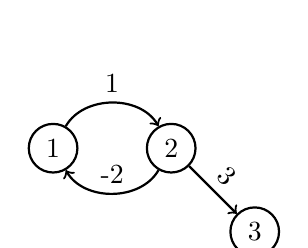
\begin{tikzpicture}[node distance={15mm}, thick, main/.style = {draw, circle}] 
    \node[main] (1) {$1$};
    \node[main] (2) [right of=1] {$2$};
    \node[main] (3) [below right of=2] {$3$};
    \draw[->] (1) to [out=60, in=120, looseness=1.0] node[midway, above]{1} (2);
    \draw[->] (2) to [out=240, in=300, looseness =1.0] node[midway, above]{-2} (1);
    \draw[->] (2) -- node[midway, above, sloped]{3} (3);
  \end{tikzpicture}
  \hspace*{\fill}
  \caption{Sample negative weight-loop.}
  \label{figure:negativeWeightLoop}
\end{figure}

\begin{algorithm}
  \caption{Bellman-Ford single source shortest path algorithm.}
  \label{algorithm:bfsssp}
  %Documentation for algorithmicx: https://texdoc.org/serve/algorithmicx/0
  \begin{algorithmic}[1]
    \Procedure{BellmanFord}{$graph$, $weightFunction$, $sourceVertex$}
      \State $InitSingleSource(graph, sourceVertex)$ \Comment{Initialize the vertices to do the algorithm}
      \For{$i \gets 0,~i < length(graph.vertices) - 1,~i++$}
        \For{$edge~\epsilon~graph.edges$} \Comment{Iterate through all the edges}
          \State $Relax(edge.fromVertex,~edge.toVertex,~weightFunction)$ \Comment{Make a better decision if needed}
        \EndFor
      \EndFor
      \State $out \gets true$ \Comment{Assume all went well}
      \For{$edge~\epsilon~graph.edges$}
        \If{$edge.toVertex.distance > edge.fromVertex.distance + weightFunction(edge.fromVertex, edge.toVertex)$}
          \State $out \gets false$ \Comment{There is a negative weight loop, so the algorithm failed}
        \EndIf
      \EndFor
      \State \Return{$out$}
    \EndProcedure

    \Procedure{InitSingleSource}{$graph$, $sourceVertex$}
      \For{$vertex~\epsilon~graph.vertices$}
        \State $vertex.distance \gets \infty$ \Comment{Assume each vertex has no path to the source}
        \State $vertex.predecessor \gets null$
      \EndFor
      \State $sourceVertex.distance \gets 0$ \Comment{The source vertex has a distance of 0 to itself}
    \EndProcedure

    \Procedure{Relax}{$fromVertex$, $toVertex$ $weightFunction$}
      \If{$toVertex.distance > fromVertex.distance + weightFunction(fromVertex, toVertex)$}
        \State $toVertex.distance \gets fromVertex.distance + weightFunction(fromVertex, toVertex)$
        \State $toVertex.predecessor \gets fromVertex$ \Comment{There is a better route to toVertex through fromVertex}
      \EndIf
    \EndProcedure
  \end{algorithmic}
\end{algorithm}

\subsection{Asymptotic Analysis}
The C++ implementation of the Bellman-Ford algorithm can be found in Listing \ref{lst:bfsssp}. First, line 6 makes a call to the $initSingleSource$ function, which starts on line 41. In the $initSingleSource$ function there is a loop on lines 43-49 that goes through each vertex in the graph and performs a couple assignments, which run in constant time for a total of $v$ times, where v is the number of vertices in the graph. After the loop, there is an assignment to make the special initialization for the source vertex on line 51. Therefore, the $initSingleSource$ function runs in $O(v)$ time. Next, the loop defined on line 8 iterates the number of vertices minus 1 times. Inside of this loop contains 2 nested loops: a while-loop that goes through each vertex (defined on line 11) and a while-loop that goes through each edge for the vertex of the outer while-loop (defined on line 14). Although deceiving, these nested while-loops iterate through each edge in the graph. The only reason why there is the loop for the vertices is because the graph is represented using linked objects and the connections between the vertex objects are the edges. Inside of the inner-most loop is a call to the $relax$ function. This method is defined on lines 54-61 and contains an if-statement with some assignments, which all run in $O(1)$ time. Therefore, the nested while-loops will run in $O(e)$ time, where $e$ is the number of edges in the graph. Since the $O(e)$ loop is nested inside of a loop that runs $v - 1$ times, the overall runtime of the loop on lines 8-21 is $O(v * e)$. Lastly, the loop structure on lines 25-36 iterates through all of the edges in the graph and has a body containing only assignments and comparisons. Therefore, the final loop runs in $O(e)$ time. When putting the 3 main parts of the algorithm together, the runtime complexity of the Bellman-Ford SSSP algorithm is $O(v + v * e + e)$, which simplifies to $O(v * e)$ because $v * e$ is the dominant term in the expression.

\section{Fractional Knapsack Algorithm}
\subsection{The Algorithm}
The fractional knapsack algorithm solves the problem of maximizing the value of the objects one takes to fill up their knapsack. As displayed in Algorithm \ref{algorithm:fracKnapsack}, the solution to the fractional knapsack problem requires a greedy approach by getting the most valuable spice available at each point the algorithm. To do this, the spices are sorted by their unit price to get the most value for the amount of spice taken. The loop on lines 7-18 will continue until the knapsack is full or until there are no more spices to consider and, as previously mentioned, will take as much of the most valuable spice that is available. Since the spices are sorted ahead of time, the greedy approach of taking the local maximum value and hope it leads to a global maximum value works because the spices are not changing and the unit prices of the spices taken will continue to decrease as the algorithm is run. This ensures that the global maximum value is always achieved for any set of spices and any knapsack capacity.

\begin{algorithm}
  \caption{Fractional Knapsack algorithm.}
  \label{algorithm:fracKnapsack}
  %Documentation for algorithmicx: https://texdoc.org/serve/algorithmicx/0
  \begin{algorithmic}[1]
    \Procedure{FractionalKnapsack}{$spices$, $capacity$}
      \State $sort(spices)$ \Comment{Sort the spices by unit value, descending order}
      \State $quantityTaken \gets new~int[spices.length]$ \Comment{Store an array to keep track of how much of each spice was taken}
      \State $capacityLeft \gets capacity$ \Comment{Start with empty knapsack}
      \State $totalValue \gets 0$ \Comment{Start off with no value}
      \State $curSpiceIndex \gets 0$ \Comment{Start with most valuable spice per unit}

      \While{$capacityLeft > 0~\&\&~curSpiceIndex < spices.length$}
        \If{$capacityLeft \ge spices[curSpiceIndex].quantity$} \Comment{Enough space to take everything}
          \State $quantityTaken[curSpiceIndex] \gets spices[curSpiceIndex].quantity$
          \State $capacityLeft \gets capacityLeft - spices[curSpiceIndex].quantity$
          \State $totalValue \gets totalValue + spices[curSpiceIndex].value$ 
        \Else \Comment{Take what we can}
          \State $quantityTaken[curSpiceIndex] \gets capacityLeft$
          \State $totalValue \gets totalValue + capacityLeft * spices[curSpiceIndex].unitPrice$
          \State $capacityLeft \gets 0$
        \EndIf

        \State{$curSpiceIndex \gets curSpiceIndex + 1$} \Comment{Move on to next spice}
      \EndWhile
      \State \Return{$quantityTaken,~totalValue$}
    \EndProcedure
  \end{algorithmic}
\end{algorithm}

\subsection{Asymptotic Analysis}
Listing \ref{lst:fracKnapsack} contains the C++ implementation of the fractional knapsack algorithm. First, line 3 makes a call to a quicksort algorithm for the spices to put them in descending order by their unit prices, which runs in $O(s * log_2s)$ time, where $s$ is the number of spices available to be taken. Next, the loop defined on line 5 iterates through each of the knapsacks because the implementation takes in many knapsacks for testing. This loop will run $k$ times, where $k$ is the number of knapsacks. The sorting algorithm is executed before the loop because all of the knapsacks are being filled with the same data and, therefore, the sorting operation only has to be done once. Line 6 is also specific to the implementation as it dequeues the next knapsack from the queue, which is a constant time operation. Lines 9, 15, 16, and 19 all define variables to keep track of, which are all constant time operations. The small loop on lines 10-12 initializes the array to use all 0s, which is a C++ specific problem as other programming languages do this automatically, which will cause these lines to be excluded from the asymptotic analysis. Next, the loop defined on line 22 continues until the knapsack is full or until there are no more spices. The worst case scenario is when there is not enough spice to fill the knapsack, which causes the loop to run a total of $s$ times. The entire body of the loop matches what is done in Algorithm \ref{algorithm:fracKnapsack}, which is only the constant time operations of conditions and assignments. Thus, the entire loop on lines 22-43 runs in $O(s)$ time. Lastly, lines 46-62 will be excluded as they are outputting the results. Overall, for each individual knapsack, the runtime complexity is $O(s * log_2s + s)$, which is $O(s * log_2s)$ because $s * log_2s$ is the dominant term in the expression. However, the implementation runs the $O(s)$ loop $k$ times, which will cause the overall runtime complexity of the C++ implementation to become $O(s * log_2s + k * s)$.

\lstset{numbers=left, numberstyle=\tiny, stepnumber=1, numbersep=5pt}

% Colors and lstset for syntax highlighting from https://www.overleaf.com/latex/examples/syntax-highlighting-in-latex-with-the-listings-package/jxnppmxxvsvk
\definecolor{mygreen}{rgb}{0,0.6,0}
\definecolor{mygray}{rgb}{0.5,0.5,0.5}
\definecolor{mymauve}{rgb}{0.58,0,0.82}
\lstset{
  backgroundcolor=\color{white},   % choose the background color
  basicstyle=\footnotesize,        % size of fonts used for the code
  breaklines=true,                 % automatic line breaking only at whitespace
  captionpos=b,                    % sets the caption-position to bottom
  commentstyle=\color{mygreen},    % comment style
  escapeinside={\%*}{*},          % if you want to add LaTeX within your code
  keywordstyle=\color{blue},       % keyword style
  stringstyle=\color{mymauve},     % string literal style
}

\section{Appendix}
\subsection{Bellman-Ford Single Source Shortest Path Algorithm}
\lstinputlisting[caption = Bellman-Ford Single Source Shortest Path Algorithm (C++), label = lst:bfsssp, language = C++, firstline = 139, lastline = 199, firstnumber = 1]{./../graph.cpp}

\subsection{Fractional Knapsack Algorithm}
\lstinputlisting[caption = Fractional Knapsack Algorithm (C++), label = lst:fracKnapsack, language = C++, firstline = 101, lastline = 167, firstnumber = 1]{./../fractionalKnapsack.cpp}

\end{document}